\begin{figure}[tbp]
\centering
\definecolor{AFDPass}{RGB}{28,125,117}
\definecolor{AFDFail}{RGB}{190,77,62}
\definecolor{AFDMedian}{RGB}{36,86,150}
\definecolor{AFDPninetyfive}{RGB}{214,129,45}

\begin{minipage}[t]{0.48\textwidth}
\centering
\textbf{\small (a) Fidelity-gate outcomes}

\vspace{3pt}
\resizebox{\linewidth}{!}{%
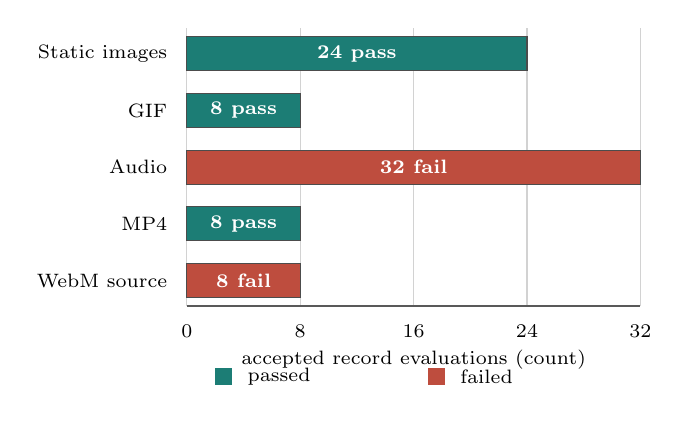
\begin{tikzpicture}[x=0.18cm,y=0.72cm,font=\scriptsize]
  \foreach \x in {0,8,16,24,32} {
    \draw[gray!35] (\x,0.55) -- (\x,5.45);
    \node[anchor=north] at (\x,0.38) {\x};
  }
  \node[anchor=east] at (-0.7,5) {Static images};
  \node[anchor=east] at (-0.7,4) {GIF};
  \node[anchor=east] at (-0.7,3) {Audio};
  \node[anchor=east] at (-0.7,2) {MP4};
  \node[anchor=east] at (-0.7,1) {WebM source};

  \filldraw[fill=AFDPass,draw=black!70] (0,4.70) rectangle (24,5.30);
  \node[text=white,font=\scriptsize\bfseries] at (12,5) {24 pass};
  \filldraw[fill=AFDPass,draw=black!70] (0,3.70) rectangle (8,4.30);
  \node[text=white,font=\scriptsize\bfseries] at (4,4) {8 pass};
  \filldraw[fill=AFDFail,draw=black!70] (0,2.70) rectangle (32,3.30);
  \node[text=white,font=\scriptsize\bfseries] at (16,3) {32 fail};
  \filldraw[fill=AFDPass,draw=black!70] (0,1.70) rectangle (8,2.30);
  \node[text=white,font=\scriptsize\bfseries] at (4,2) {8 pass};
  \filldraw[fill=AFDFail,draw=black!70] (0,0.70) rectangle (8,1.30);
  \node[text=white,font=\scriptsize\bfseries] at (4,1) {8 fail};

  \draw[black!65] (0,0.55) -- (32,0.55);
  \node[anchor=north] at (16,-0.05) {accepted record evaluations (count)};
  \fill[AFDPass] (2,-0.85) rectangle (3.2,-0.55);
  \node[anchor=west] at (3.6,-0.70) {passed};
  \fill[AFDFail] (17,-0.85) rectangle (18.2,-0.55);
  \node[anchor=west] at (18.6,-0.70) {failed};
\end{tikzpicture}%
}
\end{minipage}
\hfill
\begin{minipage}[t]{0.48\textwidth}
\centering
\textbf{\small (b) Warm latency by execution class}

\vspace{3pt}
\resizebox{\linewidth}{!}{%
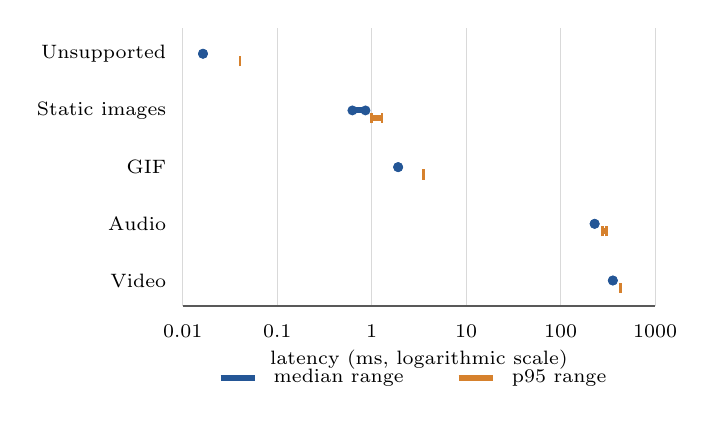
\begin{tikzpicture}[x=0.48cm,y=0.72cm,font=\scriptsize]
  % Maps latency t in milliseconds onto a log10 axis from 0.01 to 1000 ms.
  \newcommand{\latencyrange}[6]{%
    \node[anchor=east] at (-0.18,#1) {#2};
    \pgfmathsetmacro{\medianlo}{2.5*(ln(#3)/ln(10)+2)}
    \pgfmathsetmacro{\medianhi}{2.5*(ln(#4)/ln(10)+2)}
    \pgfmathsetmacro{\pninetyfivelo}{2.5*(ln(#5)/ln(10)+2)}
    \pgfmathsetmacro{\pninetyfivehi}{2.5*(ln(#6)/ln(10)+2)}
    \draw[AFDMedian,line width=2.2pt] (\medianlo,#1) -- (\medianhi,#1);
    \fill[AFDMedian] (\medianlo,#1) circle[radius=1.8pt];
    \fill[AFDMedian] (\medianhi,#1) circle[radius=1.8pt];
    \draw[AFDPninetyfive,line width=2.2pt]
      (\pninetyfivelo,{#1-0.13}) -- (\pninetyfivehi,{#1-0.13});
    \draw[AFDPninetyfive,line width=1pt]
      (\pninetyfivelo,{#1-0.22}) -- (\pninetyfivelo,{#1-0.04});
    \draw[AFDPninetyfive,line width=1pt]
      (\pninetyfivehi,{#1-0.22}) -- (\pninetyfivehi,{#1-0.04});
  }
  \foreach \x/\lab in {0/{0.01},2.5/{0.1},5/{1},7.5/{10},10/{100},12.5/{1000}} {
    \draw[gray!30] (\x,0.55) -- (\x,5.45);
    \node[anchor=north] at (\x,0.38) {\lab};
  }

  \latencyrange{5}{Unsupported}{0.016}{0.016}{0.040}{0.040}
  \latencyrange{4}{Static images}{0.625}{0.860}{0.998}{1.284}
  \latencyrange{3}{GIF}{1.906}{1.906}{3.561}{3.561}
  \latencyrange{2}{Audio}{228.799}{228.975}{279.765}{304.897}
  \latencyrange{1}{Video}{356.371}{357.113}{432.328}{433.799}

  \draw[black!65] (0,0.55) -- (12.5,0.55);
  \node[anchor=north] at (6.25,-0.05) {latency (ms, logarithmic scale)};
  \draw[AFDMedian,line width=2.2pt] (1.0,-0.72) -- (1.9,-0.72);
  \node[anchor=west] at (2.15,-0.72) {median range};
  \draw[AFDPninetyfive,line width=2.2pt] (7.3,-0.72) -- (8.2,-0.72);
  \node[anchor=west] at (8.45,-0.72) {p95 range};
\end{tikzpicture}%
}
\end{minipage}

\caption{Fidelity outcomes by source or metric group and warm latency by
execution class. Panel (a) reports 80 accepted record-level evaluations
representing 40 unique output digests. Panel (b) reports the range of profile
medians and p95 values within each execution class across 1,560 repeated warm
calls, equal to 104 records times five repetitions times three shortened
sessions. The logarithmic axis separates immediate rejection, in-process
reconstruction, and external codec paths. The observations describe this
generated corpus and host only.}
\label{fig:server-experiment-profile-results}
\end{figure}
